\section{Monochromator\_curved: A curved mosaic crystal with
a single scattering vector}
\label{s:monochromator_curved}
\index{Optics!Monochromator, curved}

%\component{Monochromator\_curved}{(System) Peter Link, FRM-2}{$z_{\rm w}$, $y_{\rm h}$, gap, $\eta_{\rm h}$, $\eta_{\rm v}$, $n_{\rm h}$, $n_{\rm v}$, $R_0$, $Q$, $r_{\rm h}$, $r_{\rm v}$}{$d_{\rm m}$, $\eta$, $h$, $w$, verbose, transmit, reflect}{In reflecting geometry, non polarized}
\mcdoccomp{optics/Monochromator_curved.parms}

\begin{figure}
  \begin{center}
    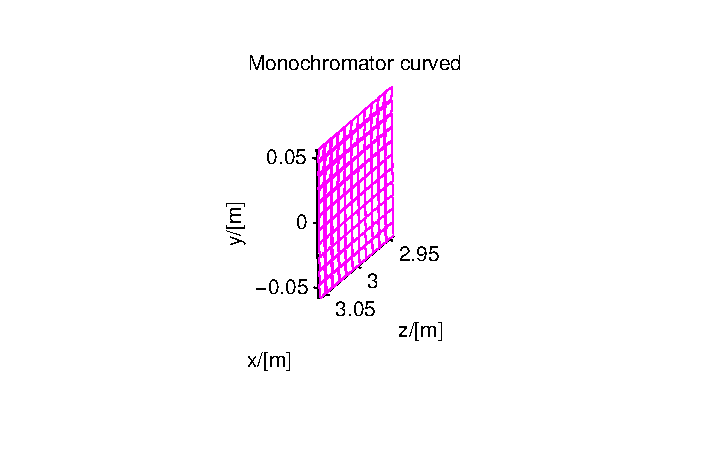
\includegraphics[width=0.9\textwidth]{figures/monochromator_curved}
  \end{center}
\caption{A curved monochromator}
\label{f:monochromator_curved}
\end{figure}


This component simulates an array of infinitely thin single
crystals with a single scattering vector perpendicular to the
surface and a mosaic spread.
This component is used to simulate a singly or doubly
curved monochromator or analyzer in reflecting geometry.

The component uses rectangular pieces of monochromator material
as described in {\bf Monochromator\_curved}.
The scattering vector is named $Q$, and as described in
{\bf Monochromator\_flat}, multiples of $Q$ will be applied.
Other important parameters are the piece height and width,
$y_{\rm h}$ and $z_{\rm w}$, respectively, the
horizontal and vertical mosaicities, $\eta_{\rm h}$ and $\eta_{\rm v}$,
respectively.
If just one mosaicity, $\eta$, is specified, this the same for both directions.

The number of pieces vertically and horizontally are called
$n_{\rm v}$ and $n_{\rm h}$, respectively, and the vertical and horizontal
radii of curvature are named $r_{\rm v}$ and $r_{\rm h}$, respectively.
All single crystals are positioned in the same vertical plane,
but tilted accordingly to the curvature radius.

The constant monochromator reflectivity, $R_0$ can be replaced by
a file of tabulated reflectivities $reflect$ (\verb+*.rfl+ in \verb+MCSTAS/data+). In the same sense, the transmission
can be modeled by a tabulated file $transmit$ (for non-reflected neutrons, \verb+*.trm+ in \verb+MCSTAS/data+).
The most useful of these files for Monochromator\_curved are \verb+HOPG.rlf+ and \verb+HOPG.trm+.

As for {\bf Monochromator\_flat}, the crystal is assumed to be infinitely
thin, and the variation in lattice spacing, ($\Delta d/d$),
is assumed to be zero. Hence, this
component is not suitable for simulating backscattering instruments or to
investigate multiple scattering effects.

The theory and algorithm for scattering from
the individual blades is described under {\bf Monochromator\_flat}.
